\section{Indledning}

% Projektbeskrivelse
\subsection{Projektbeskrivelse}
Da belysning af en bolig er afhængigt af både præferencer og indretning, er ingen lampes belysning eller udformning optimal for alle. At kunne automatisere lysstyring med en regulerbar lampe inden for både lysstyrke og position vil derfor være en praktisk løsning. Det er dog stadig vigtigt, at brugeren manuelt har mulighed for at styre lampen.

Ideen med projektet er en lampe, der hænger fra loftet i et skinnesystem, som vil kunne køre rundt til alle positioner i boligen i x-, y- og z-aksen. Lampen har et tilhørende grafisk interface i form af en touchskærm placeret i rummet, hvorpå brugeren kan kontrollere lampen og dens indstillinger. To motorer, en i hver sideskinne, styrer en tværskinnes position i rummets x-akse. Yderligere er to motor monteret på lampens base, som styrer lampens position på tværskinnen i y-aksen. Desuden vil en femte motor, monteret i lampens base, være i stand til at ændre lampens position i z-aksen (højden). Det grafiske interface, der tilbyder regulering af lampens position, har et display med 4 pile til at positionere i x- og y-aksen, samt 2 pile til z-aksen.
Systemet har 3 sensorer. En lyssensor, en afstandssensor og en bevægelsessensor. Lyssensoren har til formål at måle mængden af lys i rummet og korrigere derefter, således at lampen er i stand til at regulere sin lysstyrke efter rummets allerede tilstedeværende lys. Lampens lys er bestående af farvegivende LED’er (RGB). En afstandssensor monteret på lampens nederste kant holder øje med afstanden til nærmeste objekt for at undgå kollision. Bevægelsessensoren vurderer om der er mennesker (bevægelse) i rummet og tænder lyset når bevægelse registreres (såfremt denne funktionalitet er aktiv).

% Projektdefinition
\subsection{Projektdefinition}
Til beskrivelse af lampens funktionalitet er der udtænkt følgende systemkrav:
\begin{enumerate}
    \item I systemet skal der styres både belysning, position og behandling af indkommende sensor data. 
    \item Systemet skal kunne styres af en bruger fra et GUI.
    \item Systemet skal kunne detektere lysniveauet i et rum i lumen.
    \item Systemet skal kunne detektere afstanden fra lampens nederste kant til nærmeste objekt i z-aksen.
    \item Systemet skal kunne detektere bevægelse i rummet.
\end{enumerate}

% Systemskitse
\subsection{Systemskitse}

% 3D Koncept
\begin{figure}[H] \centering
    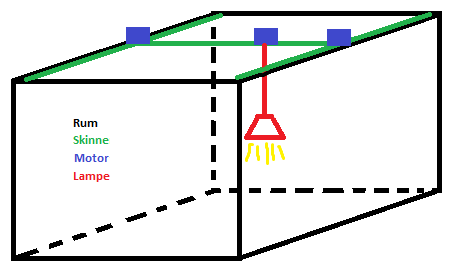
\includegraphics[width=\textwidth]{0_Filer/Figuer/3D_Koncept.png}
    \caption{3D Koncept}
    \label{fig:3Dkoncept}
\end{figure}

% Grafisk Fremstilling af Projekt
\begin{figure}[H] \centering
    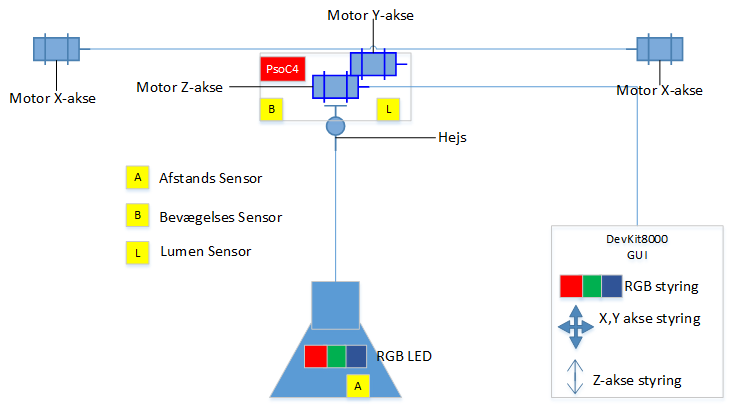
\includegraphics[width=\textwidth]{0_Filer/Figuer/Grafisk_Fremstilling_af_Projekt.png}
    \caption{Grafisk Fremstilling af Projekt}
    \label{fig:GrafiskFremstillingAfProjekt}
\end{figure}